%!TEX root = ../dokumentation.tex

\chapter{Grundlagen}
In dem folgenden Kapitel werden die Grundlagen dieser Arbeit beschrieben. Zuerst wird das in dieser Arbeit verwendete \acs{VR}-Headset vorgestellt. Nach dem \acs{VR}-Headset folgt der Eye Tracker und zum Schluss die Laufzeit- und Entwicklungsumgebung Unity.

\section{\acl{VR}}
Der Begriff \ac{VR} oder Virtuelle Realität ist eine Technik, die beschreibt wie 

\section{\acs{VR}-Headset}
Im Rahmen dieser Arbeit wird das \acs{VR}-Headset HTC Vive verwendet. Das Headset wurde gemeinsam von den Firmen HTC und Valve entwickelt. Das \acs{VR}-Headset lässt sich in die folgenden 3 Teile unterteilen. 

\cite{Clay_Koenig_Koenig_2019}
\subsection{\acl{HMD}}
Das \ac{HMD} ist 
\todo{Abbildung von Headset}

\subsection{Controller}
\todo{Abbildung von Controller}

\subsection{Lighthouse Tracking System}
\todo{Abbildung von Basisstation}

\section{Eyetracking}
Eyetracking ist eine Technologie, die erkennt, in welche Richtung eine Person ihren Blick richtet. Hierfür werden beim Eyetracking Blick sowie Augenbewegungen erfasst. Die hauptsächlichen Parameter, die durch das Eyetracking erfasst werden, sind Fixiationen, Sakkaden und Regression.

\begin{figure}[!htbp]
	\centering
	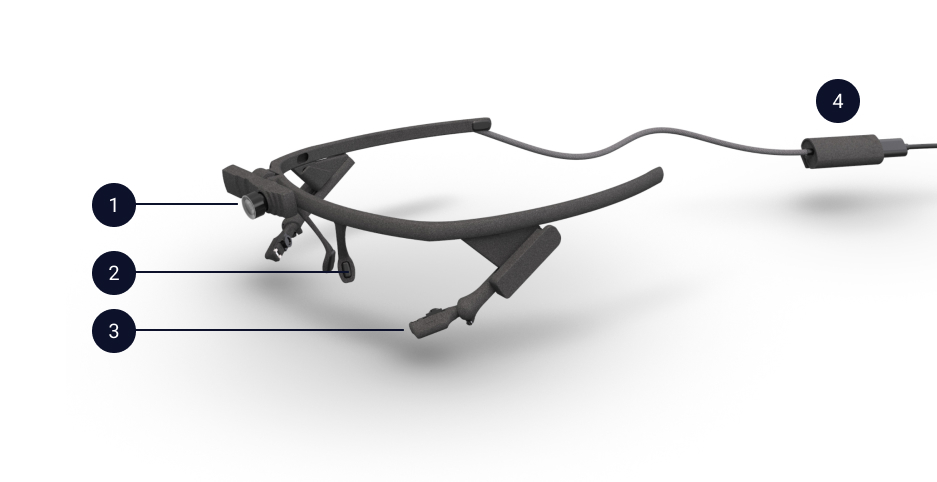
\includegraphics[width=1\linewidth]{pupil_labs_headset}
	\caption{Pupil Core Headset}
	\label{fig:pupil_labs_headset}
\end{figure}

\todo{Quelle aus Pupil Labs Dokumentation --> Core --> Hardware}

Im Rahmen dieser Arbeit wird ein Eyetracker von Pupil Labs verwendet. Sie entwickeln seit 2014 die Plattform Pupil Core, die aus einer Open-Soure-Suite sowie dem Eyetracker selber besteht. In \autoref{fig:pupil_labs_headset} ist das tragbare Eyetracker Headset Pupil Core zu sehen, welches wie eine Brille getragen wird. An dem Headset ist eine Blickfeldkamera (Nummer 1) angebracht, welche das Blickfeld des Benutzers aufnimmt. Mithilfe der Augenkameras (Nummer 3) lässt sich das komplette Auge erfassen. Die Augenkameras lassen sich individuell auf die Augen einstellen. Ein USB-C Kabel (Nummer 4) dient als Stromversorgung sowie für den Austausch der Videodaten der Kameras. Wird der Eyetracker mit dem Computer verbunden, dann lässt sich mit der Pupil Core Software das Eyetracking starten. Die Pupil Core Software beinhaltet die Programme Pupil Capture, Pupil Player und Pupil Service.

\subsection{Pupil Capture}
Das Programm Pupil Capture erfasst den Stream der Videodaten und zeigt die Videos auf dem Computer an. Aus den Videos der Augenkameras erkennt die Software die Pupillen und verfolgt den Blick des Benutzers. Im Blickfeldvideo wird der 
Aus der Pupille und des Blickes wird der Punkt berechnet, der vom Benutzer des Eyetrackers angeschaut wird. Dieser berechnete Punkt wird in das Weltvideo angezeigt.

\subsection{Pupil Player}
Mit Pupil Player lassen sich die aufgezeichneten Videos abspielen und die zugehörigen Daten Visualisieren

\subsection{Pupil Service}
Das Programm Pupil Service ist ähnlich zu Pupil Capture. Der einzige Unterschied ist, dass keine Videodaten aus der Umgebungskamera ausgewertet werden und das Programm selber keine GUI besitzt. Dieses Programm ist konzipiert für VR- und AR-Anwendungen.

\cite{PaperPupilLabs}

\section{Unity}

\subsection{steamVR}

\subsection{hmd\_eyes}